\begin{document}
\title{Distributed Systems}
\subtitle{University of Cambridge\\Computer Science Tripos, Part IB\\Michaelmas term 2020/21}
\author{Martin Kleppmann}
\institute{Department of Computer Science and Technology\\University of Cambridge}
\date{}
\maketitle

\section{Introduction}

\begin{frame}
    \label{s:title}
    \begin{center}
        \textbf{\huge{\color{darkblue}{Distributed Systems}}} \\[2em]
        The second half of \emph{Concurrent and Distributed Systems}\\[0.5em]
        \href{https://www.cl.cam.ac.uk/teaching/current/ConcDisSys/}{www.cl.cam.ac.uk/teaching/current/ConcDisSys/}\\[2em]
        Martin Kleppmann (mk428@cam) \\[0.5em]
        University of Cambridge \\[0.5em]
        Computer Science Tripos, Part IB \\[0.5em]
        Michaelmas term 2020/21 \\[0.5em]
    \end{center}
\end{frame}

This 8-lecture course on distributed systems forms the second half of \emph{Concurrent and Distributed Systems}.
While the first half focussed on concurrency among multiple processes or threads running on the same computer, this second half takes things further by examining systems consisting of multiple communicating computers.

Concurrency on a single computer is also known as \emph{shared-memory concurrency}, since multiple threads running in the same process have access to the same address space.
Thus, data can easily be passed from one thread to another: a variable or pointer that is valid for one thread is also valid for another.

This situation changes when we move to distributed systems.
We still have concurrency in a distributed system, since different computers can execute programs in parallel.
However, we don't typically have shared memory, since each computer in a distributed system runs its own operating system with its own address space, using the memory built into that computer.
Different computers can only communicate by sending each other messages over a network.

(Limited forms of distributed shared memory exist in some supercomputers and research systems, and there are technologies like \emph{remote direct memory access} (RDMA) that allow computers to access each others' memory over a network.
Also, databases can in some sense be regarded as shared memory, but with a different data model compared to byte-addressable memory.
Broadly speaking, and most practical distributed systems are based on message-passing.)

\begin{frame}
    \label{s:dist-sys-definition}
    \frametitle{A distributed system is\dots}
    \begin{itemize}
        \item<1-> \emph{``{\dots}a system in which the failure of a computer you didn't even know existed can render your own computer unusable.''} --- Leslie Lamport\\[1em]
        \item<2> {\dots}multiple computers communicating via a network\dots
        \item<2> {\dots}trying to achieve some task together
    \end{itemize}
    \hfill\includegraphics<1>[height=4cm]{images/lamport.jpg}
\end{frame}
\inlineslide{s:dist-sys-definition}\label{l:dist-sys-definition}
% reference for Lamport quote: https://www.microsoft.com/en-us/research/publication/distribution/

There are a number of reasons for creating distributed systems.
Some applications are instrinsically distributed: if you want to send a message from your phone to your friends' phones, that operation inevitably requires that those phones communicate via some kind of network.

In other cases, we use distributed systems to do things that can in principle be done on a single computer, but using a distributed system allows us to do it \emph{better}.
For example, ``better'' might mean ``more reliable'': a single computer can fail and might need to be rebooted from time to time, but if you are using multiple computers, then if one of them fails, another can take over.
Thus, a distributed system has the potential to be more reliable than a single computer, at least if it is well-designed (somewhat contradicting Lamport's quote on Slide~\ref{l:dist-sys-definition})!

Another reason for using distribution is for better performance: if a service has users all over the world, and they all have to access a single computer, then either the users in the UK or the users in New Zealand are going to find it slow (or both).
By placing computers around the world, we can get around the slowness of the speed of light by routing each user to a nearby computer.

Finally, some large-scale data processing or computing tasks are simply too big to perform on a single computer, or would be intolerably slow.
For example, the Large Hadron Collider at CERN is supported by a worldwide computing infrastructure with 1 million CPU cores for data analysis, and 1 exabyte ($10^{18}$ bytes) of storage! See \url{https://wlcg-public.web.cern.ch/}.

\begin{frame}
    \label{s:why-distribute}
    \frametitle{Why make a system distributed?}
    \begin{itemize}\pause
        \item \textbf{It's inherently distributed:}\\e.g. sending a message from your mobile phone to your friends' phones\pause
        \item \textbf{For better reliability:}\\even if one computer fails, the system as a whole keeps functioning\pause
        \item \textbf{For better performance:}\\get data from a nearby computer rather than one halfway round the world\pause
        \item \textbf{To solve bigger problems:}\\e.g. huge amounts of data, can't fit on one machine
    \end{itemize}
\end{frame}
\inlineslide{s:why-distribute}

However, there are also downsides to distributed systems, because things can go wrong, and the system needs to deal with such faults.
For example, the network may go down, making the computers unable to communicate.

\begin{frame}
    \label{s:no-internet}
    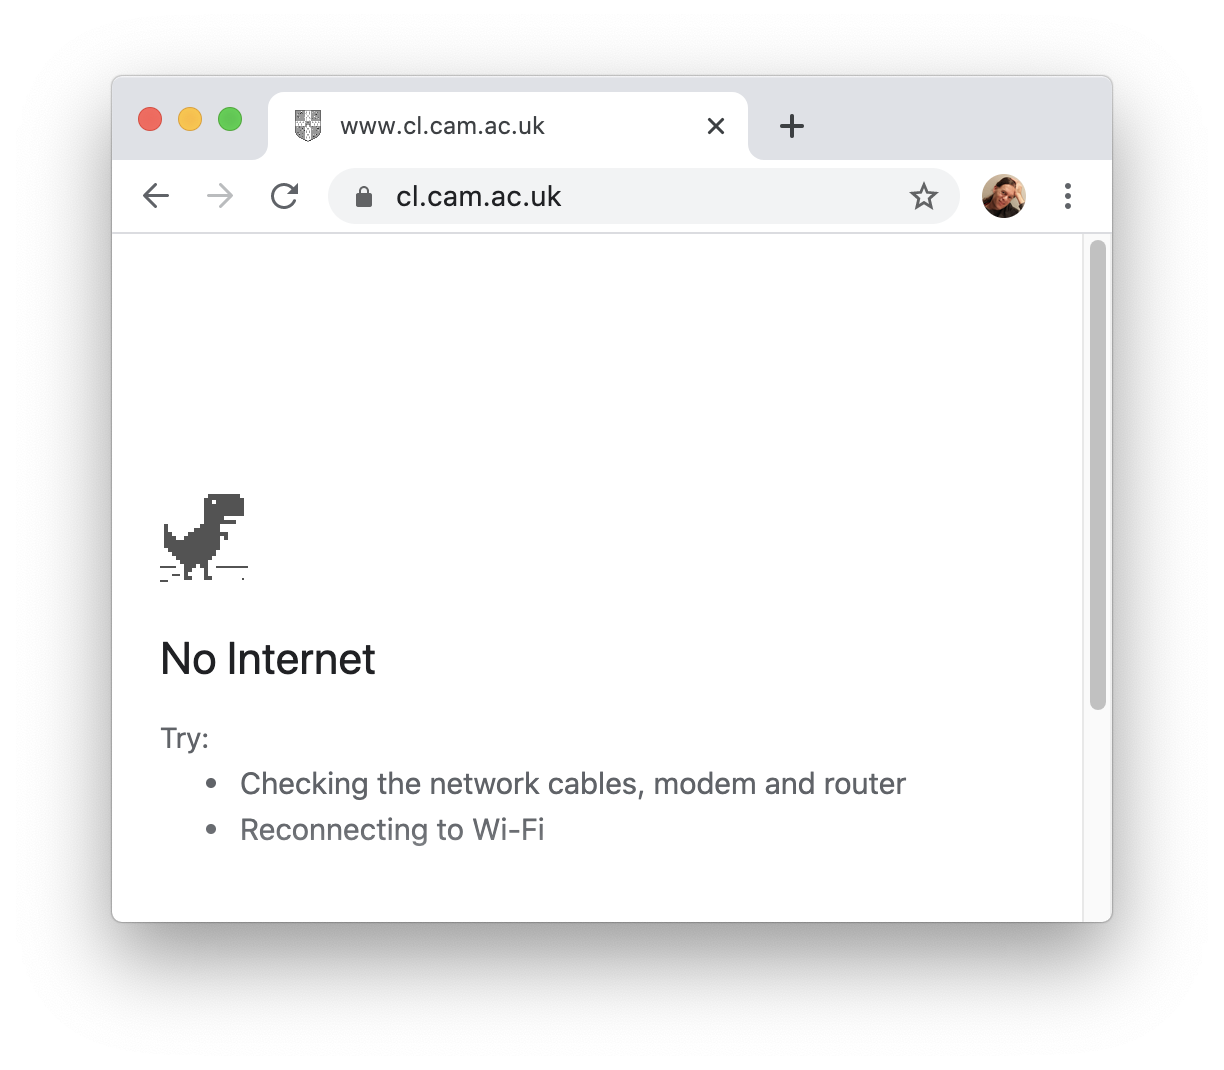
\includegraphics[height=\paperheight]{images/no-internet.png}
\end{frame}
\inlineslide{s:no-internet}

For example, one of the computers crashes and another needs to take over.
This requires detecting that a crash has happened; as we shall see, even that is not straightforward.

Say one of the RAM modules fails in a computer: we don't expect the computer to continue working nevertheless.
It will probably just crash.
However, in a distributed system we often \emph{do} want to tolerate some parts of the system being broken, and for the rest to continue working.


\begin{frame}
    \label{s:why-not}
    \frametitle{Why NOT make a system distributed?}
    The trouble with distributed systems:
    \begin{itemize}
        \item Communication may fail (and we might not even know it has failed).
        \item Processes may crash (and we might not know).
        \item All of this may happen nondeterministically.
    \end{itemize}\vspace{1em}
    Dealing with this is hard.\\[1em]
    Writing a program to run on a single computer is comparatively easy?!
\end{frame}
\inlineslide{s:why-not}

\begin{frame}
    \label{s:reading}
    \frametitle{Recommended reading}
    \begin{itemize}
        \item Coulouris et al.\\ ``\textbf{Distributed Systems: Concepts and Design}''\\(5th ed), Addison-Wesley 2012
        \item Tanenbaum et al.\\ ``\textbf{Distributed Systems: Principles and Paradigms}''\\(2nd ed), Prentice Hall 2006 
        \item Kleppmann.\\ ``\textbf{Designing Data-Intensive Applications}'',\\O’Reilly 2017
        \item Bacon \& Harris.\\ ``\textbf{Operating Systems: Concurrent and Distributed Software Design}'', Addison-Wesley 2003
    \end{itemize}
\end{frame}
\inlineslide{s:reading}

\begin{frame}
    \label{s:other-courses}
    \frametitle{Relationships with other courses}
    \begin{itemize}
        \item \textbf{Concurrent Systems} -- Part IB\\
            (every distributed system is also concurrent)
        \item \textbf{Operating Systems} -- Part IA\\
            (inter-process communication, scheduling)
        \item \textbf{Databases} -- Part IA\\
            (many modern databases are distributed)
        \item \textbf{Computer Networking} -- Part IB Lent term\\
            (distributed systems involve network communication)
        \item \textbf{Further Java} -- Part IB Michaelmas\\
            (distributed programming practical exercises)
        \item \textbf{Security} -- Part IB Easter term\\
            (network protocols with encryption \& authentication)
        \item \textbf{Cloud Computing} -- Part II\\
            (distributed systems for processing large amounts of data)
    \end{itemize}
\end{frame}
\inlineslide{s:other-courses}

\begin{frame}
    \label{s:networking}
    \frametitle{Distributed Systems and Computer Networking}
    We use a simple abstraction of communication:
    \begin{center}
        \begin{tikzpicture}
            \node [circle,fill=red!10,draw] (i) at (0,0) {node $i$};
            \node [circle,fill=red!10,draw] (j) at (6,0) {node $j$};
            \draw [bigarrow] (i) -- node [above] {message $m$} (j);
        \end{tikzpicture}
    \end{center}

    Reality is much more complex:
    \begin{itemize}
        \item \textbf{Various network operators:}\\ eduroam, home DSL, cellular data, coffee shop wifi, submarine cable, satellite\dots\\[1em]
        \item \textbf{Physical communication:}\\ electric current, radio waves, laser, hard drives in a van\dots
    \end{itemize}
\end{frame}
\inlineslide{s:networking}

Relationship between dist sys and networking: networking is how you get the bytes ``over the wire'' (or over the wireless network) to another machine; dist sys is what you do with the bytes once they get there.
We don't care about the ``bits on the wire''.

The ``wire'' may actually be radio waves, lasers, hard drives in a van, or even a USB thumb drive in someone's pocket
% AWS Snowball: https://docs.aws.amazon.com/snowball/latest/ug/using-device.html

Fundamental abstraction: nodes (or processes); sending a message from one node to another.

\begin{frame}[plain]
    \label{s:snowball}
    \frametitle{Hard drives in a van?!}
    \begin{center}
        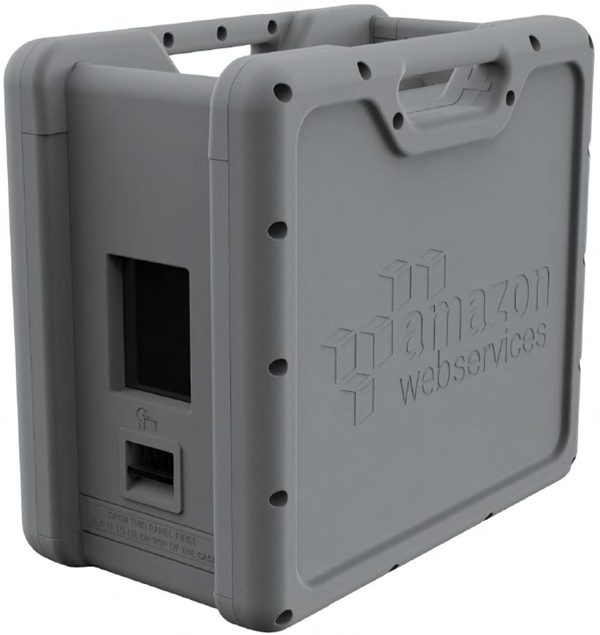
\includegraphics[height=5cm]{images/aws-snowball.png}\\[0.5em]
        \footnotesize{\url{https://docs.aws.amazon.com/snowball/latest/ug/using-device.html}}
    \end{center}
\end{frame}
\inlineslide{s:snowball}

\section{Models of distributed systems}

``reliability'' of TCP; screenshots of network error + request timeout

Why distribute?
- Inherently distributed: communication, collaboration (Facebook, google docs).
- Scale, performance, fault tolerance

It's easy if you can do it on one machine! Don't distribute unless you have to. 

Distributed systems are fascinating because we have to work with partial knowledge and uncertain
truths. We never have certainty about the state of the system, because by the time we hear about
something, that state may already be outdated. In this way it resembles real life more than most of
computing! In real life you need to often make decisions with incomplete information.

Two generals problem, Byzantine generals problem
% two generals: https://link.springer.com/chapter/10.1007/3-540-08755-9_9

Calendar app supports offline reads and writes (short video in airplane mode).

\begin{itemize}
\item synchronous, partially synchronous~\cite{Dwork:1988dr}, and asynchronous model
\item crash-stop, crash-recovery, and arbitrary (Byzantine) faults
\item network may drop, duplicate, reorder packets (and even sniff and spoof?)
\end{itemize}

network message delay: synchronous, partially synchronous, asynchronous

network reliability: reliable, fair-loss, arbitrary. (fair-loss means non-zero probability of a
given message being delivered. links guarantee messages not created out of thin air -- see Cachin et al.
Arbitrary links need authentication.)

can we make a fair-loss link reliable? send acknowledgements and retransmit on timeout; deduplicate
on recipient side. however, in crash-recovery model, retry and deduplication state would be lost on
crash, so this needs to be maintained in stable storage.

Fundamental building blocks of distributed systems: replication and partitioning.

Replication example: two clients A and B, four servers. Server 1 receives only A's request,
server 2 receives A then B, server 3 receives B then A, and server 4 receives only B.
How do we ensure replicas become consistent with each other?

Use this as motivation for introducing causality and happens-before.
Show that physical timestamp ordering may  be inconsistent with causality.
Distinguish between A and B being concurrent, and A happening before B
(determining which one should overwrite the other).

ABD algorithm. Last writer wins. Linearizability.

notion of causality: taken from physics (relativity).
When a happened before b, that doesn't mean that a necessarily caused b; it just means that a \emph{might have} caused b.
For this reason, we sometimes say that the happens-before relationship encodes \emph{potential causality}.

However, when a and b happened independently (no message sent after a arrived before b, and no message sent after b arrived before a), we know that a \emph{cannot have caused} b and vice versa.

Hybrid Logical Clocks - Kulkarni et al, Logical physical clocks (OPODIS 2014) \url{https://doi.org/10.1007/978-3-319-14472-6_2}

Exercise. A relation R is a strict partial order if it is transitive ($\forall a,b,c.\; (a,b) \in R \wedge (b,c) \in R \Longrightarrow (a,c) \in R$) and irreflexive ($\nexists a.\; (a,a) \in R$). Show that the happens-before relation is a strict partial order.

Exercise. Show that for any two events $a$ and $b$, exactly one of the three following statements must be true: either $a \rightarrow b$, or $b \rightarrow a$, or $a \parallel b$.

% 1. Network communication basics: JSON, TCP, HTTP/REST, UDP. Hands-on: using things like tcpdump?
% 2. Faults and failures
% 3. Architectures: client-server, local networks (multicast), peer-to-peer (distributed hash tables, NAT traversal)
% 4. Programming models: services, RPC, message brokers, actors, map-reduce, stream processing, tuple spaces?
% 5. Replication
% 6. Consensus
% 7. Convergence
% 8. Time and clocks
% 9. Security (e.g. TLS), byzantine fault tolerance, and blockchains

% Live demo of RESTful API with Dropwizard, curl, browser access

% State machine replication

% "causality is reachability in spacetime"
% https://twitter.com/palvaro/status/1233208997257170944

% message loss -> retry; duplicates -> detect and suppress duplicates / idempotence
% idempotence: f(f(x)) = f(x)
% incrementing number of likes on a post: not idempotent
% adding current user to the set of users who have liked a post: idempotent
% what state must a recipient maintain in order to eliminate duplicates?
% the entire message? a unique message ID? a sequence number? (what assumptions does this require making about the sender?)

% MIT graduate dist-sys course https://pdos.csail.mit.edu/6.824/schedule.html
% Raft animations: http://thesecretlivesofdata.com/raft/

\bibliographystyle{plainurl}
\bibliography{references}{}
\end{document}
